% Copyright Aidan Randle-Conde 2007-2014
% http://www.aidansean.com/phd_notes
% Anyone is free to download, redistribute, edit and use these notes and the source tex files with the following restrictions:
% This 
%  This message is included in the tex source files.
%  Aidan Randle-Conde is credited as the author.
%  Images are correctly credited to their respective authors, as outlined in the references.
%  No part of these notes may be used for commercial purposes.

\chapter{Quantum chromodynamics (QCD)}
\chaptermark{Quantum chromodynamics}

\section{Deep inelastic scattering}

Quantum chromodynamics gives rise to gluons with trilinear and quadrilinear couplings.

\begin{figure}[!htb]
  \begin{center}
    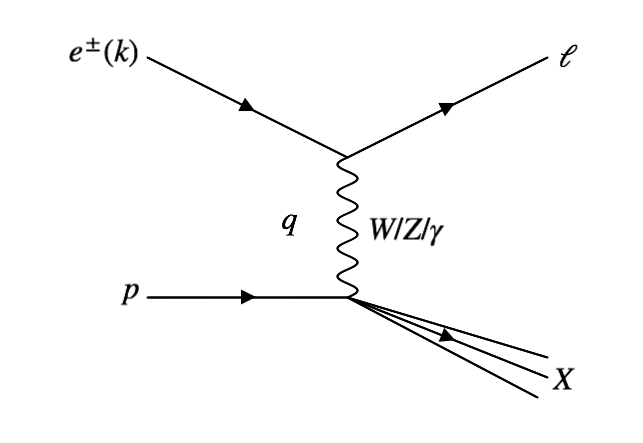
\includegraphics[width=0.8\textwidth]{images/web_feynman/image_60.png}
    \caption[Deep inelastic scattering]{Deep inelastic scattering.}
    \label{fig:ch14_DIS}
  \end{center}
\end{figure}

For such a process the following dimensionless variables are defined:

\begin{eqnarray*}
  x & = & \frac{-q}{2p \cdot q} \\
  & = & \frac{Q^2}{2p \cdot q} \\
  y & = & \frac{q \cdot p}{k \cdot p}
\end{eqnarray*}

At the proton vertex:

\begin{eqnarray*}
  q + p & = & p_H \\
  \Rightarrow p_H^2 & = & q^2 + p^2 + 2p \cdot q \\
  m_H^2 & = & q^2 + 2p \cdot q + m_p^2
\end{eqnarray*}

So $m_H$ is a function of the invariant $Q^2$ and $2p \cdot q$ and $x$ is the ratio of the invariants, characterising the hadronic vertex.

Historically the ignorance of the hadron vertex was/is described by structure functions which multiply all the invariant kinematic quantities.

It is known that the probes, $\gamma$, $W^{\pm}$, $Z^0$, interact with quarks and antiquarks in the proton and neutron.  The quarks and antiquarks interact with gluons, which carry around $50\%$ of the four-momentum.  The nucleon is a QCD system of quarks, antiquarks and gluons interacting with each other.  So the DIS cross-sections are calculated, using the scattering of leptonic probes by the quark antiquark constituents and later modify results to take into account the quark gluon interaction.

\section{The quark-parton model}

$x$ in the quark-parton model:

\begin{figure}[!htb]
  \begin{center}
    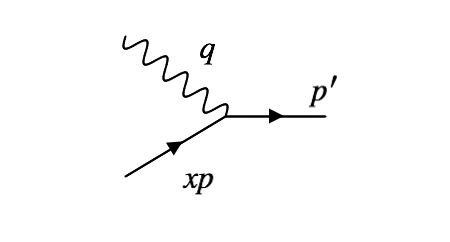
\includegraphics[width=0.8\textwidth]{images/web_feynman/image_61.png}
    \caption[Quark-parton scattering]{Quark-parton scattering.}
    \label{fig:ch14_quarkPartonScattering}
  \end{center}
\end{figure}

The incoming quark carries a fraction $x$ of the proton's four-momentum $p$:

\begin{eqnarray*}
  p' & = & q + xp \\
  \Rightarrow p'^2 & = & q^2 + 2xpq + x^2p^2 \\
  \textrm{for } q & >> & xp \\
  q^2 & >> & m_H^2 \\
  0 & = & q^2 + 2xq \cdot p \\
  \Rightarrow x & = & \frac{-q^2}{2q \cdot p}
\end{eqnarray*}

The centre of mass energy in the centre of mass system, $\sqrt{\hat{s}}$, is:

\begin{figure}[!htb]
  \begin{center}
    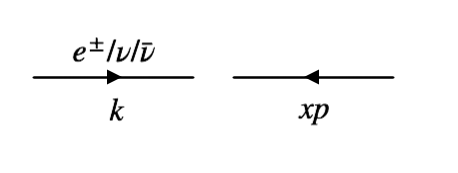
\includegraphics[width=0.5\textwidth]{images/web_feynman/image_62.png}
    \caption[CM deep inelastic scattering]{Deep inelastic scattering in the centre of mass frame.}
    \label{fig:ch14_DISCM}
  \end{center}
\end{figure}

\begin{eqnarray*}
  s & = & \left(k + p\right)^2 \\
  & \simeq & 2k \cdot p \\
  \textrm{for } s & >> & \left(m_p\right)^2 \\
  \hat{s} & = & \left(k + xp\right)^2 \\
  & \simeq & 2xk \cdot p \\
  & = & xs \\
  y & = & \frac{q \cdot p}{k \cdot p} \\
  & = & \frac{\left(k - k'\right) \cdot px}{k \cdot xp} \\
  & = & 1 - \frac{k' \cdot xp}{k \cdot xp} \\
  & = & \frac{1 - E'Eq - |E'||E|\left(-\cos\theta\right)}{E'Eq - |E'||Eq|\left(-1\right)} \\
  & = & 1 - \left(\frac{1 + \cos\theta}{2}\right) \\
  & = & \frac{1 - \cos\theta}{2}
\end{eqnarray*}

\begin{figure}[!htb]
  \begin{center}
    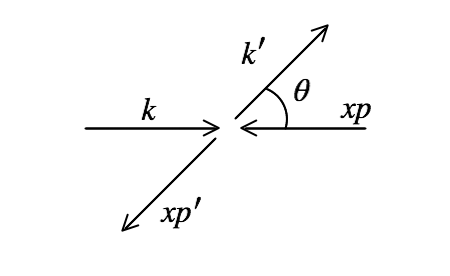
\includegraphics[width=0.75\textwidth]{images/web_feynman/image_63.png}
    \caption[Deep inelastic scattering variables]{Definitions of deep inelastic scattering variables $k$, $k'$, $p$, and $p'$.}
    \label{fig:ch14_DISVariables}
  \end{center}
\end{figure}

$y = 1$ signifies a very deeply inelastic collision and occurs when $\cos\theta = -1$.

The expression for $\e^+\e^-$ scattering off a nucleon via photon can be determined by analogy with $\e\mu$ scattering:

\[
  \left.\frac{\mathrm{d}\sigma}{\mathrm{d}\Omega}\right|_{\e\mu} = \frac{1}{64\pi^2\hat{s}}2\e^4\left(\frac{\hat{s}^2 + \hat{u}^2}{\hat{t}^2}\right)
\]

For quarks, replace $\e^4$ by $\e^4\left(q_i\right)^2$ where $q_i = -1/3$, $2/3$.

\begin{eqnarray*}
  y & = & \frac{1 - \cos\theta}{2} \\
  \Rightarrow \mathrm{d}y & = & \frac{-\mathrm{d}\cos\theta}{2} \\
  \textrm{so } \frac{\mathrm{d}\sigma}{\mathrm{d}\Omega} & = & \frac{\mathrm{d}\sigma}{2\pi\mathrm{d}\left(\cos\theta\right)} \\
  & = & \frac{1}{64\pi\hat{s}}2\e^4q_i^2\Bigg[ \frac{\hat{s}^2 + \hat{u}^2}{\hat{t}^2}\Bigg] \\
  \Rightarrow \frac{\mathrm{d}\sigma}{4\pi\mathrm{d}y} & = & \frac{1}{64\pi^2\hat{s}Q^2}2\e^4q_i^2\hat{s}^2\Bigg[ 1 + \frac{\hat{u}^2}{\hat{s}^2}\Bigg] \\ 
  \textrm{so } \frac{\mathrm{d}\sigma}{\mathrm{d}y} & = & \frac{1}{8\pi}\frac{\e^4q_i^2}{Q^2}\hat{s}\left(1 + \left(1 - y\right)^2\right) \\
  & = & \frac{2\pi\alpha^2q_i^2}{Q^4}\hat{s}\left(1 + \left(1 - y\right)^2\right) \\
  & = & \frac{2\pi\alpha^2 q_i^2}{Q^4}\hat{s}\left(2 - 2y + y^2\right)
\end{eqnarray*}

In the nucleon the fraction of quarks having $x$ between $x'$ and $x' + \delta x'$ is $Q_i(x',Q^2) \mathrm{d}x'$ where $Q_i$ is the parton distribution function for the quark concerned.  These cannot be calculated in QCD but their evolution with $x$ and $Q^2$ can be.  The aim of DIS experiments is to measure $Q_i(x,Q^2)$ and to compare their evolution with theory:  Doshsitzer-Gribov-Lipatov-Attareli-Parisi (DGLAP) equation.

This gives:

\begin{eqnarray*}
  \left.\frac{\mathrm{d}\sigma}{\mathrm{d}y}\right|_{x'<x<x' + \delta x'} & = & \frac{2\pi\alpha^2}{Q^4}q_i^2\left(1 + \left(1 - y\right)^2\right)x'sQ(x')\mathrm{d}x' \\
  \textrm{so } \frac{\mathrm{d}\sigma}{\mathrm{d}x\mathrm{d}y} & = & \frac{2\pi\alpha^2}{Q^4}\sum_i q_i^2\left(1 + \left(1 - y\right)^2\right)s\left(xQ_i(x) + x\bar{Q}_i(x)\right)
\end{eqnarray*}

The photon interacts equally with quarks and antiquarks.  In the absence of QCD effects the $Q_i$ are functions of $x$ (known as scaling).  However QCD effects make the $Q_i$ become functions of $x$ and $Q^2$.  There is also a gluon distribution in the proton.  It is a triumph of QCD to predict this evolution.

For a neutrino beam the cross-section was calculated as:

\[
  \left.\frac{\mathrm{d}^2\sigma}{\mathrm{d}x\mathrm{d}y}\right|_{\nu} \propto \Big[xQ_d(x) + x\bar{Q}_u(x)\left(1 - y\right)^2\Big]
\]

as this is a charged current interaction with $W$ exchange.  Here particular quarks are ``picked out'' and the specific densities can be measured.

To encompass the quark densities they are written in terms of a structure function:

\[
  \frac{F_2}{x} = \sum_i Q_i(x,Q^2) + \bar{Q}_i(x,Q^2)
\]

At fixed $Q^2$ experiments determine $xQ(x)$ and $x\bar{Q}(x)$ which contain combinations of $u$, $d$, $s \cdots$ quarks.  These can be from collisions such as $\e^{\pm}p \quad \nu n$ and then all experimental points can be fed into a fit to determine $u(x)$, $d(x)$ etc.

\subsection{Drell-Yan process}

The Drell-Yan process is a quark in a proton colliding with an antiquark in an anti-proton (or proton).  In the centre of mass frame the kinematics are:

\begin{figure}[!htb]
  \begin{center}
    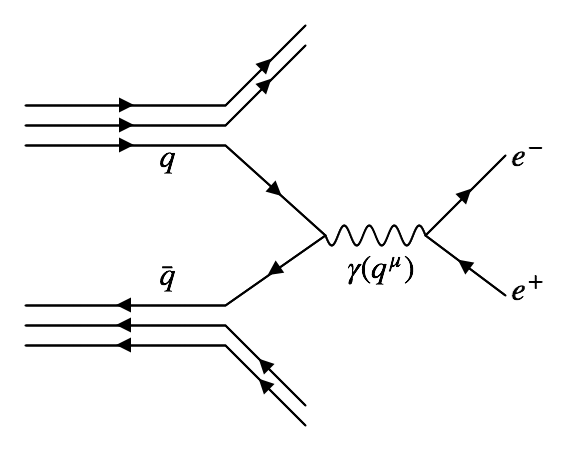
\includegraphics[width=0.75\textwidth]{images/web_feynman/image_64.png}
    \caption[Drell-Yan process]{Drell-Yan process in $p\bar{p}$ collisions.}
    \label{fig:ch14_DrellYan}
  \end{center}
\end{figure}

\begin{eqnarray*}
  x_1p_1 & = & x_1(p_1,0,0,p_1) \\
  x_2p_2 & = & x_2(p_2,0,0,-p_2) \\
  \Rightarrow q^{\mu} & = & \left(\left(x_1 + x_2\right)p,0,0,\left(x_1 - x_2\right)p\right) \\
  \textrm{Assuming } p & = & p_1 = p_2 \\
  \Rightarrow q^2 & = & \left( \left(x_1 + x_2\right)^2 - \left(x_1 - x_2\right)^2\right)p^2 \\
  & = & 4x_1x_2p^2 \\
  & = & x_1x_2s \textrm{ or } \hat{s} \\
  \textrm{Since } \sigma(\e^+\e^-\to\mu^+\mu^-) & = & \frac{4\pi\alpha^2}{3\hat{s}} \\
  \frac{\mathrm{d}^2\sigma}{\mathrm{d}x_1\mathrm{d}x_2} & = & \frac{1}{3}\frac{4\pi\alpha^2}{3\hat{s}}q_i^2\Big[Q_i(x_1)\bar{Q}_i(x_2) + \bar{Q}_i(x_1)Q_i(x_2)\Big]
\end{eqnarray*}

Many processes at colliders are Drell-Yann processes such as:

\begin{figure}[!htb]
  \begin{center}
    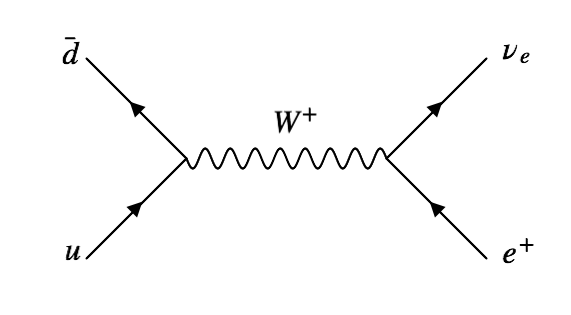
\includegraphics[width=0.75\textwidth]{images/web_feynman/image_65.png}
    \caption[Drell-Yan process $u\bar{d}\to e^+\nu_e$]{Drell-Yan process $u\bar{d}\to e^+\nu_e$.}
    \label{fig:ch14_DrellYanUDToENu}
  \end{center}
\end{figure}

The gluon distribution can be important for predicting exotic processes at the LHC, such as Higgs production:

\begin{figure}[!htb]
  \begin{center}
    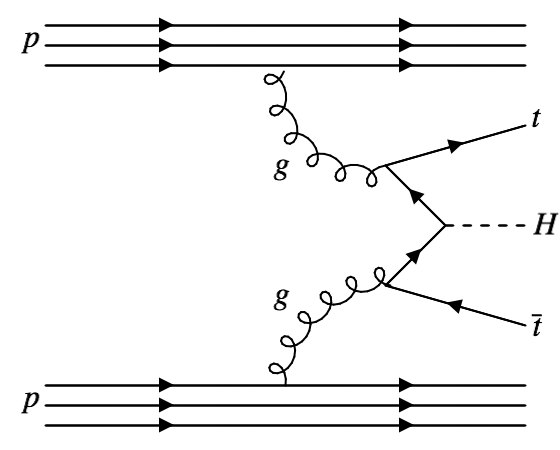
\includegraphics[width=0.75\textwidth]{images/web_feynman/image_66.png}
    \caption[$ttH$ production]{$ttH$ production at a $pp$ collider.}
    \label{fig:ch14_DrellYanUDToENu}
  \end{center}
\end{figure}

Colour interactions are assumed to be analogous to the electromagnetic interaction, so the rules of QED are used with the substitution $\alpha \to \alpha_s$.

So for $q_1 q_2 \to q_1 q_2$, $|T_{fi}|^2 = \frac{4}{9}\left(\frac{s^2 + u^2}{t^2}\right)$, which is similar to $\e\mu \to \e\mu$.

For $q_1 \bar{q}_1 \to q_1 \bar{q}_1$, $|T_{fi}|^2 = \frac{4}{9}\left(\frac{s^2 + u^2}{t^2} + \frac{t^2 + u^2}{s^2}\right) - \frac{8}{27}\frac{u^2}{st}$, which is similar to $\e^+\e^- \to \e^+\e^-$.

\subsection{The evolution of the structure function (DGLAP equations)}

The simple quark-parton model is modified by QCD Compton processes.

\begin{figure}[!htb]
  \begin{center}
    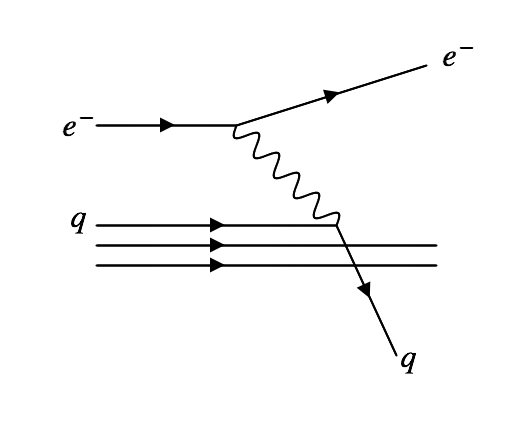
\includegraphics[width=0.75\textwidth]{images/web_feynman/image_67.png}
    \caption[Simple parton model scattering]{Simple parton model scattering.}
    \label{fig:ch14_simplePartonDIS}
  \end{center}
\end{figure}

\begin{figure}[!htb]
  \begin{center}
    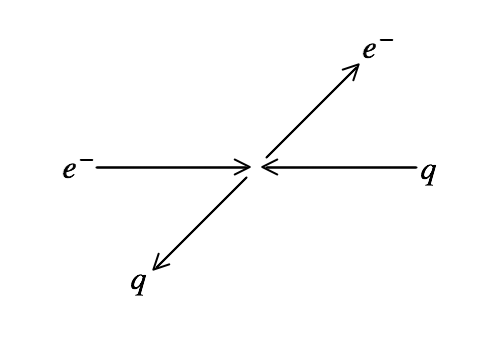
\includegraphics[width=0.5\textwidth]{images/web_feynman/image_68.png}
    \caption[$eq$ scattering in the centre of mass frame]{$eq$ scattering in the centre of mass frame.}
    \label{fig:ch14_simplePartonDISCM}
  \end{center}
\end{figure}

\begin{figure}[!htb]
  \begin{center}
    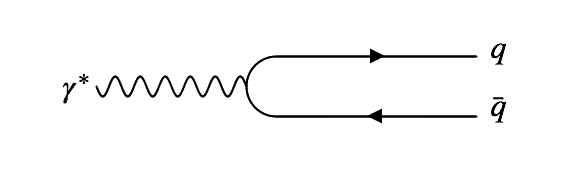
\includegraphics[width=0.5\textwidth]{images/web_feynman/image_69.png}
    \caption[Electromagnetic quark production]{Electromagnetic quark production, $\gamma\to q\bar{q}$.}
    \label{fig:ch14_simplePartonDISGammaQQ}
  \end{center}
\end{figure}

The kinematics are described by:

\begin{figure}[!htb]
  \begin{center}
    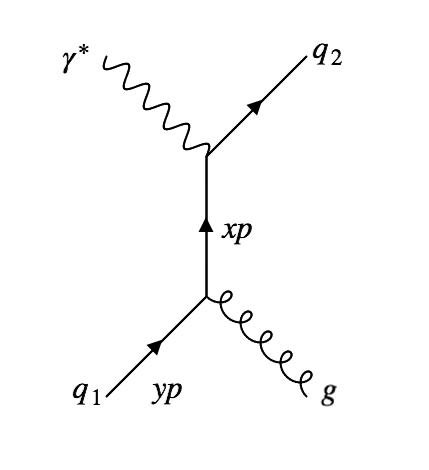
\includegraphics[width=0.5\textwidth]{images/web_feynman/image_70.png}
    \caption[Quark photon fusion process]{Quark photon fusion process, $\gamma^*q\to gq'$.}
    \label{fig:ch14_QGammaToQG}
  \end{center}
\end{figure}

\begin{eqnarray*}
  z & = & \frac{Q^2}{2q_1 \cdot q} \\
  & = & \frac{x}{y} \\
  \hat{s} & = & \left(yp + q\right)^2 \\
  & = & y^2p^2 + q^2 = 2yp \cdot q \\
  z & = & \frac{Q^2}{2y p \cdot q} \\
  \Rightarrow p \cdot q & = & \frac{Q^2}{2yz} \\
  \Rightarrow \hat{s} & = & 0 - Q^2 + \frac{Q^2}{z} \\
  & = & \frac{Q^2\left(1 - z\right)}{z}
\end{eqnarray*}

In the $\gamma^{\star}q_1$ frame:

\begin{figure}[!htb]
  \begin{center}
    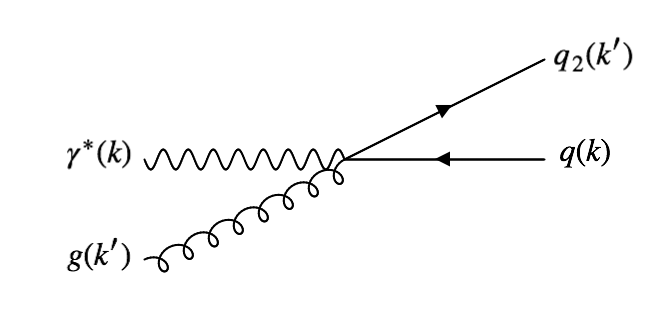
\includegraphics[width=0.5\textwidth]{images/web_feynman/image_71.png}
    \caption[CM quark photon fusion process]{Quark photon fusion process in the CM frame.}
    \label{fig:ch14_QGammaToQGCM}
  \end{center}
\end{figure}

$\ul{k}$ and $\ul{k}'$ are the $3-$momenta of the initial and final states.

\begin{eqnarray*}
  \hat{s} & = & \left(g + q_2\right)^2 \\
  & \simeq & 2g \cdot q_2 \\
  & = & 2k'k' - 2k'k'\cos(180^{\circ}) \\
  & = & 4k'^2 \\
  \hat{t} & = & \left(g - q_1\right)^2 \\
  & = & -2kk'\left(1 - \cos\theta\right) \\
  \hat{u} & = & \left(q_1 - q_2\right) \\
  & = & -2kk'\left(1 + \cos\theta\right) \\
  \textrm{Also } -\hat{u} - \hat{t} & = & 4kk' \\
  \textrm{Recall } \hat{s} + \hat{u} + \hat{t} & = & \sum p_i^2 \\
  & = & -Q^2 \\
  \Rightarrow - \hat{t} - \hat{u} & = & \hat{s} + Q^2 \\
  \Rightarrow \hat{s} + Q^2 & = & 4kk'
\end{eqnarray*}

For the virtual QED Compton process:

\begin{eqnarray*}
  \frac{\mathrm{d}\sigma}{\mathrm{d}\Omega} & = & \frac{1}{64\pi^2\hat{s}}2\e^4\Bigg[ -\frac{u}{s} - \frac{s}{u} + \frac{2tQ}{su} \Bigg] \\
  \frac{\alpha^2}{2s} & = & \frac{1}{64\pi^2\hat{s}}2\e^4
\end{eqnarray*}

Now convert this to QCD.  ie one $\gamma$ and one $g$ interchange $u$ and $t$:

\[
  \left.\frac{\mathrm{d}\sigma}{\mathrm{d}\Omega}\right|_{QCDC} = C_F\frac{\alpha\alpha_s}{2\hat{s}}\e_1^2\Bigg[ -\frac{\hat{t}}{\hat{s}} - \frac{\hat{s}}{\hat{u}} + \frac{2\hat{u}Q}{\hat{s}\hat{t}} \Bigg] 
\]

where $C_F$ is the colour factor $= 4/3$.

\begin{figure}[!htb]
  \begin{center}
    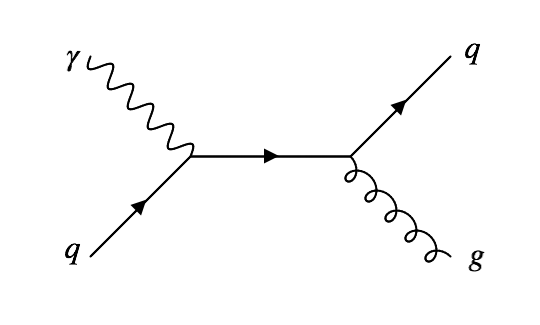
\includegraphics[width=0.5\textwidth]{images/web_feynman/image_72.png}
    \caption[Colour factor in quark photon fusion]{Colour factor in quark photon fusion.}
    \label{fig:ch14_QGammaToQGColour}
  \end{center}
\end{figure}

There are $3\times3-1$ possible colour configurations, then averaging over the number of quark colours gives a factor of $8/3$, and dividing by $2$ gives $4/3$ (due to the historical definition of $\alpha_s$).

An intersting quantity is the transverse momentum of the outgoing quark:

\begin{eqnarray*}
  p_T & = & k'\sin\theta \\
  \hat{s}\hat{t}\hat{u} & = & 4k'^2\left(-2kk'\right)\left(1 - \cos\theta\right)\left(-2kk'\right)\left(1 + \cos\theta\right) \\
  & = & 16k'^2\left(kk'\right)^2\sin^2\theta \\
  & = & 16k^2k'^2p_T^2 \\
  \textrm{Recall } s + Q^2 & = & 4kk' \\
  \Rightarrow \hat{s}\hat{t}\hat{u} & = & \left(s + Q^2\right)^2p_T^2 \\
  \textrm{So } p_T^2 & = & \frac{\hat{s}\hat{t}\hat{u}}{\left(\hat{s} + Q^2\right)^2}
\end{eqnarray*}

For small scattering angles $\cos\theta\sim 1$.

\begin{eqnarray*}
  \mathrm{d}\left(p_T^2\right) & = & k'^2\mathrm{d}\left(\sin^2\theta\right) \\
  & = & 2k'^2\sin\theta\cos\theta\mathrm{d}\theta \\
  & = & \frac{\hat{s}}{2}\sin\theta\mathrm{d}\theta \\
  \textrm{And } \mathrm{d}\Omega & = & 2\pi\sin\theta\mathrm{d}\theta \\
  \Rightarrow \mathrm{d}p_T^2 & = & \frac{\hat{s}}{2}\frac{\mathrm{d}\Omega}{2\pi} \\
  \textrm{or } \mathrm{d}\Omega & = & \frac{4\pi}{\hat{s}}\mathrm{d}p_T^2 \\
  \textrm{For } \theta \to , 0 \quad  -\hat{t} & << & \hat{s} \\
  \textrm{So } p_T^2 & = & \frac{\hat{s}\hat{t}\left(-\hat{s}-Q^2\right)}{\left(s + Q^2\right)^2} \\
  \Rightarrow \frac{\mathrm{d}\sigma}{\mathrm{d}p_T^2} & = & \frac{4\pi}{\hat{s}}\frac{4}{3}\frac{\alpha\alpha_s}{2\hat{s}}\e_i^2\Bigg[\frac{-\hat{s}}{\hat{t}} + \frac{2\hat{u}Q^2}{\hat{s}\hat{t}}\Bigg] \\
  & = & \frac{8\pi}{3}\frac{\alpha\alpha_s\e_i^2}{\hat{s}^2}\left(\frac{-1}{\hat{t}}\right)\Bigg[\hat{s} + \frac{2\left(\hat{s} + Q^2\right)Q^2}{\hat{s}}\Bigg] \\
  & = & \frac{4\pi^2\alpha}{\hat{s}}\frac{2\alpha_s}{3\pi}\frac{\e_i^2}{\hat{s}}\frac{\hat{s}}{p_T^2\left(\hat{s} + Q^2\right)}\Bigg[ \hat{s} + \frac{2\left(\hat{s} + Q^2\right)Q^2}{\hat{s}}\Bigg] \\
  & = & \sigma_0 \frac{2\alpha_s}{3\pi}\e_i^2\frac{1}{p_T^2}\Bigg[\frac{\hat{s}}{\hat{s}+Q^2} + \frac{2Q^2}{\hat{s}} \Bigg] \\
  & = & \sigma_0\frac{2\alpha_s}{3\pi}\e_i^2\frac{1}{p_T^2}\Bigg[\frac{\hat{s}^2 + 2Q^2\left(\hat{s} + Q^2\right)}{\left(\hat{s} + Q^2\right)\hat{s}}\Bigg] \\
  & = & \e_i^2\sigma_0\frac{1}{p_T^2}\frac{\alpha_s}{2\pi}p_{qq}(z)
\end{eqnarray*}

where $\sigma_0 = \frac{4\pi^2\alpha}{\hat{s}}$ is the $\gamma^{\star} p$ total cross-section and $p_{qq}(z) = \frac{4}{3}\left(\frac{1 + z^2}{1 - z}\right)$ which is the probability of a quark emitting a gluon and so becoming a quark with momentum reduced by a fraction $z$.

\begin{eqnarray*}
  \Rightarrow \hat{\sigma}(\gamma q \to gq) & = & \int_{\mu^2}^{\frac{\hat{s}}{4}}\mathrm{d}p_T^2\frac{\mathrm{d}\hat{\sigma}}{\mathrm{d}p_T^2} \\
  & = & \e_i^2 \int_{\mu^2}^{\frac{\hat{s}}{4}}\frac{\mathrm{d}p_T^2}{p_T^2}\frac{\alpha_s}{2\pi}P_{qq}(z)
\end{eqnarray*}

where $\mu^2$ is a cut-off so that the integral is not divergent as $p_T^2 \to 0$.

\begin{eqnarray*}
  \sigma & = & \e_i^2\hat{\sigma}_0\frac{\alpha_s}{2\pi}p_{qq}(z)\ln\left(\frac{Q^2}{\mu^2}\right) \\
\textrm{where  }\left.p_T^2\right|_{max} & = & \frac{\hat{s}}{4} = \frac{Q^2(1 - z)}{4z}
\end{eqnarray*}

At large $Q^2$: $\ln Q^2 + \ln\left(\frac{1-z}{4z}\right) \sim \ln Q^2$.

\begin{figure}[!htb]
  \begin{center}
    \begin{tabular}{rl}
      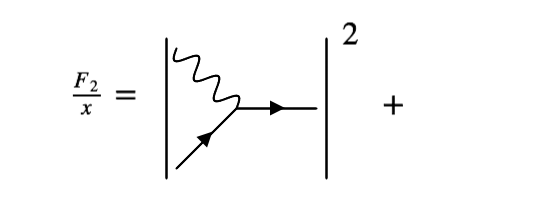
\includegraphics[width=0.5\textwidth]{images/web_feynman/image_73a.png} &
      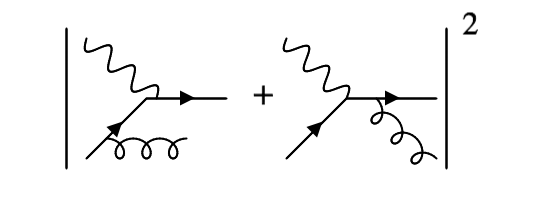
\includegraphics[width=0.5\textwidth]{images/web_feynman/image_73b.png}
    \end{tabular}
    \caption[Structure function for large $Q^2$]{Structure function, $F_2$, for large $Q^2$.}
    \label{fig:ch14_F2}
  \end{center}
\end{figure}

\[
  \Rightarrow \frac{F_2}{x} = \sum_q \e_q^2 \int_x^1 \frac{\mathrm{d}y}{y}Q(y)\Bigg[ \delta\left(1 - \frac{x}{y}\right) + \frac{\alpha_s}{2\pi}P_{qq}\left(\frac{x}{y}\right)\ln\left(\frac{Q^2}{\mu^2}\right)\Bigg]
\]

where $Q(y)$ is the probability that there is a quark of a certain momentum.  The presence of $Q^2$ means that the parton model scaling no longer holds and $F_2$ is a function of $Q^2$ as well as $x$.  This equation can be thought of as the start of a power series in $\alpha_s$.

\begin{eqnarray*}
  \frac{F_2(x,Q^2)}{x} & = & \sum_q \e_q^2 \left(Q(x) + \Delta Q(x,Q^2)\right) \\
  \textrm{and } \frac{\mathrm{d}}{\mathrm{d}\ln Q^2}\left(Q(x,Q^2)\right) & = & \frac{\alpha_s}{2\pi}\int_x^1\frac{\mathrm{d}y}{y}Q(y,Q^2)P_{qq}\left(\frac{x}{y}\right)
\end{eqnarray*}

As $Q^2$ increases the probe gains a higher resolution and can observe softer quarks in the structure $Q(x)$.

\begin{figure}[!htb]
  \begin{center}
    \begin{tabular}{rl}
      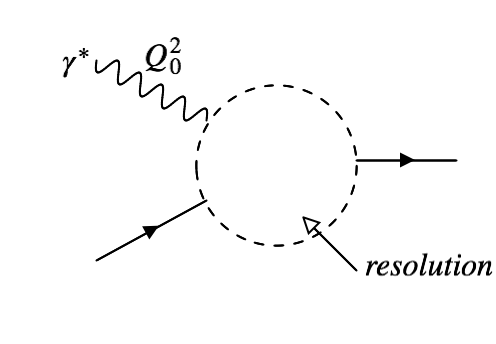
\includegraphics[width=0.5\textwidth]{images/web_feynman/image_74.png} &
      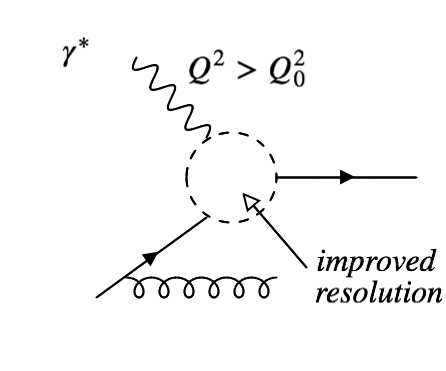
\includegraphics[width=0.5\textwidth]{images/web_feynman/image_75.png}
    \end{tabular}
    \caption[Change of resolution with $Q^2$]{Change of resolution with $Q^2$.}
    \label{fig:ch14_resolution}
  \end{center}
\end{figure}

\subsection{Boson-gluon fusion (BGF)}

$\left.\frac{F_2(x,Q^2)}{x}\right|_{\gamma^{\star}g \to q\bar{q}}$ has two intefering components:

\begin{figure}[!htb]
  \begin{center}
    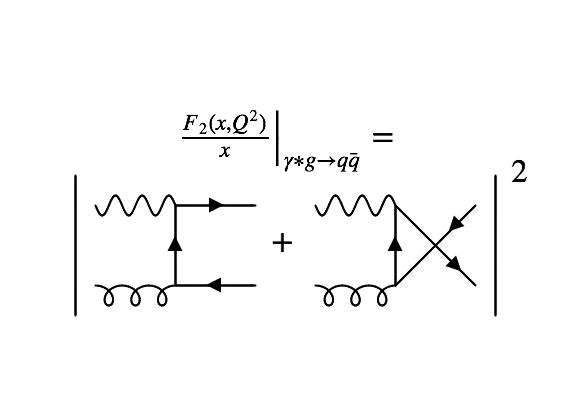
\includegraphics[width=\textwidth]{images/web_feynman/image_76.png}
    \caption[Boson-gluon fusions processes]{Boson-gluon fusions processes.}
    \label{fig:ch14_BGF}
  \end{center}
\end{figure}

\begin{eqnarray*}
  \left.\frac{\mathrm{d}\sigma}{\mathrm{d}\Omega}\right|_{BGF} & = & \frac{1}{4}\frac{\e_i^2\alpha\alpha_s}{s}\Bigg[\frac{u}{t} + \frac{t}{u} - \frac{2sQ^2}{tu}\Bigg] \\
  \left.\frac{F_2(x,Q^2)}{x}\right|_{\gamma^{\star}g \to q\bar{q}} & = & \sum_q \e_q^2 \int_x^1 \frac{\mathrm{d}y}{y}G(y)\frac{\alpha_s}{2\pi}P_{qg}\left(\frac{x}{y}\right)\ln\left(\frac{Q^2}{\mu^2}\right)
\end{eqnarray*}

where $G(y)$ is the gluon density in the proton and

\[
  P_{qg} = \frac{1}{2}\left(z^2 + (1 - z)^2\right)
\]

is the probability that a gluon annihilates into a $q\bar{q}$ pair.

\begin{eqnarray*}
  \textrm{So } \frac{\mathrm{d}Q_i(x,Q^2)}{\mathrm{d}\ln Q^2} & = & \frac{\alpha_s}{2 \pi}\int_x^1 \frac{\mathrm{d}y}{y}\left(Q_i(y,Q^2)P_{qq}\left(\frac{x}{y}\right) + G(y,Q^2)P_{qg}\left(\frac{x}{y}\right)\right) \\
  \frac{\mathrm{d}G(x,Q^2)}{\mathrm{d}\ln Q^2} & = & \frac{\alpha_s}{2\pi}\int_x^1\frac{\mathrm{d}y}{y}\left(Q_i(y,Q^2)P_{gq}\left(\frac{x}{y}\right) + G(y,Q^2)P_{gg}\left(\frac{x}{y}\right)\right)
\end{eqnarray*}

These are leading order in $\alpha_s$ functions and there are, of course, higher orders.

Although this has been derived for, and confirmed in DIS experiments, this is simply the parton structure of the proton.  It should be universal and for a given $x$ and $Q^2$ of a proton in any collision, $F_2$ has a specific value.
